\documentclass[11pt]{article}
\usepackage{color, array, graphics}
\usepackage{amsmath}
\usepackage{amssymb}
\usepackage{enumerate}
\usepackage{mathtools}
\usepackage{fullpage}
\usepackage{graphicx}
\usepackage{float}
\usepackage{listings}
\usepackage[utf8]{inputenc}

\begin{document}
\lstset{stringstyle=\ttfamily,
	showstringspaces=false,
	basicstyle=\small}

\begin{center} Alexander Garcia \hfill June 19, 2017 \\ Assignment-4 \end{center}

\medskip

\begin{enumerate}

	\item Data: $[(0,0),(1,1),(2,3)]$

		\begin{enumerate}[(a)]

			\item A full degree polynomial interpolation using the Lagrange basis is by definition

			\[
				y = \sum_{i = 1}^{n} y_i L_i(x_i)
			\]
			where
			\[
				L_i = \prod_{k = 1\ k \neq i}^{n} \frac{x-x_k}{x_i-x_k}
			\] \

			In this case, $n=3$ and

			\begin{tabular}{lll}
				$x_1 = 0$ & $x_2 = 1$ & $x_3 = 2$ \\
				$y_1 = 0$ & $y_2 = 1$ & $y_3 = 3$ \\
			\end{tabular} \\

			$y = 0L_1(x_1) + 1L_2(x_2) + 3L_3(x_3)$

			\[
				L_2 = \frac{x-0}{1-0} * \frac{x-2}{1-2}
				= -x^2 + 2x
			\]

			\[
				L_3 = \frac{x-0}{2-0} * \frac{x-1}{2-1}
				= \frac{x^2-x}{2}
			\]

			\[
				y = -x^2 + 2x + \frac{3}{2}(x^2-x) = \frac{1}{2}(x^2 + x)
			\]

			Just to ensure the interpolant agrees with the data, a small MATLAB script was used to plot $y$ with the points
			overlaid.

			\begin{center}
				\texttt{holmes5\_1.m} script
			\end{center}
			\lstinputlisting{holmes5_1.m} \

			\begin{figure}[H]
				\centering
				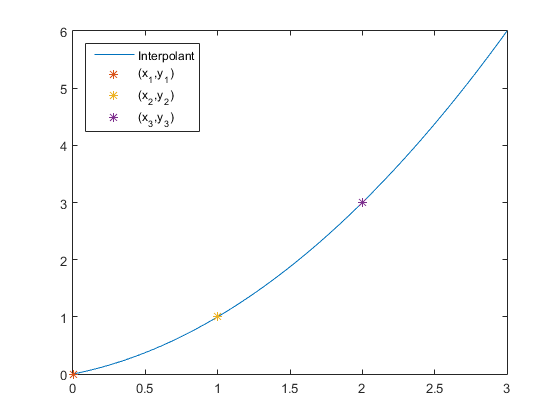
\includegraphics[width=0.5\textwidth]{holmes5_1.png}
				\caption{Graph of $y$ and the data points}
			\end{figure} \

			\item Piecewise linear interpolation for this data set consists of 2 equations $S_1(x), S_2(x)$ which
				interpolate the data between $[x_1, x_2]$, $[x_2, x_3]$ respectively.

				In general, $$S_i(x) = a_ix+b_i$$ where $$S_i(x_i) = y_i$$ From here, we get
				$$a_i = \frac{y_{i+1}-y_i}{x_{i+1}-x_i}\ \ \ \ \ b_i = y_i - \frac{y_{i+1}-y_i}{x_{i+1}-x_i}*x_i$$

				Then,
				\[
					S_1(x) = \frac{1-0}{1-0}x + (0-\frac{1-0}{1-0}*0)
					=x\ \ \ \ \ x\in[0,1]
				\]

				and
				\[
					S_2(x) = \frac{3-1}{2-1}x + (1-\frac{3-1}{2-1}*1)
					=2x - 1\ \ \ \ \ x\in[1,2]
				\]

				A simple script \texttt{holmes5\_1\_lin.m} was used to check the results of the interpolation.

				\begin{center}
					\texttt{holmes5\_1\_lin.m}
				\end{center}
				\lstinputlisting{holmes5_1_lin.m}

				\begin{figure}[H]
					\centering
					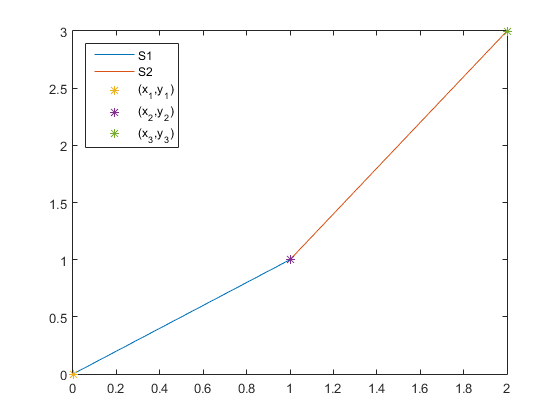
\includegraphics[width=0.5\textwidth]{holmes5_1_lin.png}
					\caption{Graph of linear piecewise interpolant}
				\end{figure} \

			\item Natural cubic spline interpolation insists that the second derivative at both the first and last data points
				are zero.

				Again, there are 2 equations $S_1(x), S_2(x)$ that interpolate the data between $[x_1, x_2]$, $[x_2,x_3]$
				respectively. In general, $$S_i(x) = a_ix^3 + b_ix^2+c_ix+d_i$$
				In order to satisfy the interpolation conditions, it must be enforced that $S_i(x_i) = y_i$. In addition, to
				ensure a smooth curve through the data, we insist that $S_i(x_i) = S_{i+1}(x_i),\ S'_i(x_i) = S'_{i+1}(x_i),\
				S''_i(x_i) = S''_{i+1}(x_i)$

				Given the initial conditions, we can construct a matrix to solve for the coefficients $a_i, b_i, c_i, d_i$.
				Each entry in matrix $\mathbf{A}$ is the value of $x_i$ raised to the corresponding power.

				\[
					\begin{bmatrix}
						0 & 0 & 0 & 1 & 0 & 0 & 0 & 0\\
						1 & 1 & 1 & 1 & 0 & 0 & 0 & 0\\
						0 & 0 & 0 & 0 & 1 & 1 & 1 & 1\\
						0 & 0 & 0 & 0 & 8 & 4 & 2 & 1\\
						6 & 2 & 0 & 0 &-6 &-2 & 0 & 0\\
						3 & 2 & 1 & 0 &-3 &-2 &-1 & 0\\
						0 & 2 & 0 & 0 & 0 & 0 & 0 & 0\\
						0 & 0 & 0 & 0 &12 & 4 & 0 & 0\\
					\end{bmatrix}
					\begin{bmatrix}
						a_1 \\
						b_1 \\
						c_1 \\
						d_1 \\
						a_2 \\
						b_2 \\
						c_2 \\
						d_2 \\
					\end{bmatrix}
					=
					\begin{bmatrix}
						0 \\
						1 \\
						1 \\
						3 \\
						0 \\
						0 \\
						0 \\
						0 \\
					\end{bmatrix}
				\] \\

				A brief explanation of the contents of this matrix:

				\begin{tabular}{cl}
					Rows 1-4: & Interpolation conditions; $S_i(x_i) = y_i$ \\
					Rows 5-6: & ``Smoothness'' conditions; agreeing first and second derivatives \\
					Rows 7-8: & Natural spline conditions; zero end point second derivatives \\
				\end{tabular} \

				Solving this system using the backslash command in MATLAB yields

				\[
					\mathbf{c}=
					\begin{bmatrix}
						0 & 0 & 1 & 0 & 1 & -3 & 4 & -1 \\
					\end{bmatrix}^T
				\]

				Using these results, we have $$S_1(x) = x$$ and $$S_2(x) = x^3 - 3x^2 + 4x - 1$$
				Below is the script used to both calculate and plot the resulting splines.

				\begin{center}
					\texttt{holmes5\_1\_cubic.m}
				\end{center}
				\lstinputlisting{holmes5_1_cubic.m} \

				\begin{figure}[H]
					\centering
					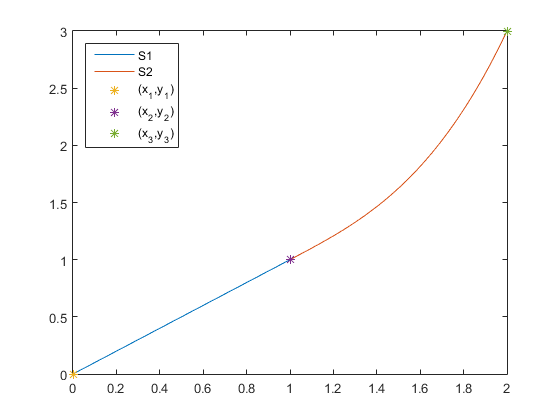
\includegraphics[width=0.5\textwidth]{holmes5_1_cubic.png}
					\caption{Graph of cubic piecewise interpolant}
				\end{figure} \

		\end{enumerate}

	\item Function to interpolate: $f(x) = sinx$

		\begin{enumerate}[(a)]

			\item Piecewise linear interpolation

				The linear spline passing through $\frac{\pi}{8}$ would be $S_1(x)$.
				$$S_1(x) = \frac{y_2-y_1}{x_2-x_1}x + (y_1 - \frac{y_2-y_1}{x_2-x_1})x_1\ \ \ \ x\in[0,\frac{\pi}{4}]$$
				$$S_1(x) = \frac{\sqrt{2}/2-0}{\pi/4-0}x + (\sqrt{2}/2 - \frac{\sqrt{2}/2-0}{\pi/4-0})0$$
				$$= \frac{\sqrt{2}/2}{\pi/4}x$$

				A MATLAB script \texttt{holmes5\_5a.m} was used to calculate the estimated value of $f(\pi/8)$, and plot
				the interpolant and the original function.

				$$S_1(\pi/8) = 0.35355$$
				$$|S_1(\pi/8) - sin(\pi/8)| = 0.02913$$ \\

				\begin{center}
					\texttt{holmes5\_5a.m}
				\end{center}
				\lstinputlisting{holmes5_5a.m} \

				\begin{figure}[H]
					\centering
					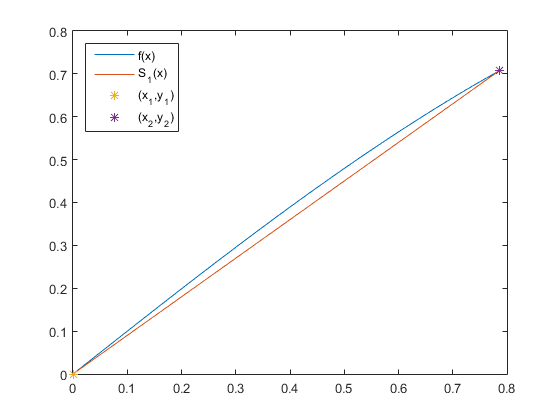
\includegraphics[width=0.5\textwidth]{holmes5_5a.png}
					\caption{Graph of $f(x)$ and $S_1(x)$}
				\end{figure} \

			\item Full degree interpolation using the Lagrange basis

				The Lagrange interpolant in this case uses $n = 3$, with data points

				\begin{tabular}{lll}
					$x_1 = 0$ & $x_2 = \frac{\pi}{4}$ & $x_3 = \frac{\pi}{2}$ \\
					$y_1 = 0$ & $y_2 = \frac{\sqrt{2}}{2}$ & $y_3 = 1$ \\
				\end{tabular}

				$y = 0L_1(x_1) + (\sqrt{2}/2)L_2(x_2) + 1L_3(x_3)$

				\[
					L_2(x_2) = \frac{x-0}{\pi/4-0}*\frac{x-\pi/2}{\pi/4-\pi/2}
					= -\frac{16x^2-8\pi x}{\pi^2}
				\]

				\[
					L_3(x_3) = \frac{x-0}{\pi/2-0} * \frac{x-\pi/4}{\pi/2-\pi/4}
					= \frac{8x^2-2\pi x}{\pi^2}
				\]

				\[
					y = -\frac{\sqrt{2}}{2}*\frac{16x^2-8\pi x}{\pi^2} + \frac{8x^2-2\pi x}{\pi^2}
					= \frac{(8-8\sqrt{2})x^2+(4\sqrt{2}\pi-2\pi)x}{\pi^2}
				\]

				Again, MATLAB was used to verify the result, as well as calculate the error.

				$$y(\pi/8) = 0.40533$$
				$$|y(\pi/8)-sin(\pi/8)| = 0.02265$$ \\

				\begin{center}
					\texttt{holmes5\_5b.m}
				\end{center}
				\lstinputlisting{holmes5_5b.m} \

				\begin{figure}[H]
					\centering
					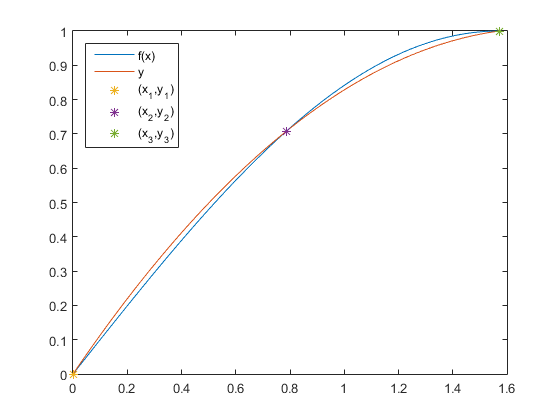
\includegraphics[width=0.5\textwidth]{holmes5_5b.png}
					\caption{Graph of $f(x)$ and full degree interpolating polynomial $y$}
				\end{figure} \

			\item Natural cubic spline interpolation \\

				\begin{tabular}{cl}
					Rows 1-4: & Interpolation conditions; $S_i(x_i) = y_i$ \\
					Rows 5-6: & ``Smoothness'' conditions; agreeing first and second derivatives \\
					Rows 7-8: & Natural spline conditions; zero end point second derivatives \\
				\end{tabular} \\

				\[
					\begin{bmatrix}
						0 & 0 & 0 & 1 & 0 & 0 & 0 & 0\\
						\pi^3/64 & \pi^2/16 & \pi/4 & 1 & 0 & 0 & 0 & 0\\
						0 & 0 & 0 & 0 & \pi^3/64 & \pi^2/16 & \pi/4 & 1\\
						0 & 0 & 0 & 0 & \pi^3/8 & \pi^2/4 & \pi/2 & 1\\
						3\pi^2/16 & \pi/2 & 1 & 0 & -3\pi^2/16 & -\pi/2 & -1 & 0\\
						3\pi/2 & 2 & 0 & 0 & -3\pi/2 & -2 & 0 & 0\\
						0 & 2 & 0 & 0 & 0 & 0 & 0 & 0\\
						0 & 0 & 0 & 0 & 3\pi & 2 & 0 & 0\\
					\end{bmatrix}
					\begin{bmatrix}
						a_1\\
						b_1\\
						c_1\\
						d_1\\
						a_2\\
						b_2\\
						c_2\\
						d_2\\
					\end{bmatrix}
					=
					\begin{bmatrix}
						0\\
						\sqrt{2}/2\\
						\sqrt{2}/2\\
						1\\
						0\\
						0\\
						0\\
						0\\
					\end{bmatrix}
				\] \\

				A MATLAB script was used to calculate the resulting coefficients, the error of the interpolating spline,
				as well as plot the spline and $f(x)$. The resulting splines are \\

				\begin{center}
				\begin{tabular}{lr}
					$S_1(x) = -0.21374x^3 + 1.03216x$ & $x\in[0,\pi/4]$ \\
					$S_2(x) = 0.21374x^3 - 1.00725x^2 + 1.82325x - 0.20711$ & $x\in[\pi/4,\pi/2]$ \\
				\end{tabular}
				\end{center}

				$$S_1(\pi/8) = 0.39239$$
				$$|S_1(\pi/8) - sin(\pi/8)| = 0.00970$$ \\

				\begin{center}
					\texttt{holmes5\_5c.m} script
				\end{center}
				\lstinputlisting{holmes5_5c.m} \

				\begin{figure}[H]
					\centering
					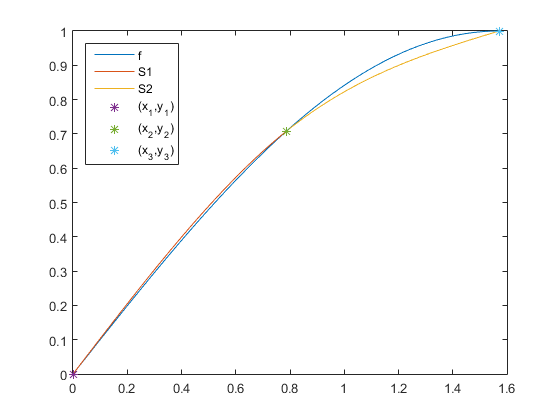
\includegraphics[width=0.5\textwidth]{holmes5_5c.png}
					\caption{Graph of $f(x)$ and natural cubic splines $S_1(x), S_2(x)$}
				\end{figure} \

			\item Clamped cubic spline interpolation \\

				\begin{tabular}{cl}
					Rows 1-4: & Interpolation conditions; $S_i(x_i) = y_i$ \\
					Rows 5-6: & ``Smoothness'' conditions; agreeing first and second derivatives \\
					Rows 7-8: & Clamped spline conditions; fixed end point first derivatives \\
				\end{tabular} \\

				\[
					\begin{bmatrix}
						0 & 0 & 0 & 1 & 0 & 0 & 0 & 0\\
						\pi^3/64 & \pi^2/16 & \pi/4 & 1 & 0 & 0 & 0 & 0\\
						0 & 0 & 0 & 0 & \pi^3/64 & \pi^2/16 & \pi/4 & 1\\
						0 & 0 & 0 & 0 & \pi^3/8 & \pi^2/4 & \pi/2 & 1\\
						3\pi^2/16 & \pi/2 & 1 & 0 & -3\pi^2/16 & -\pi/2 & -1 & 0\\
						3\pi/2 & 2 & 0 & 0 & -3\pi/2 & -2 & 0 & 0\\
						0 & 0 & 1 & 0 & 0 & 0 & 0 & 0\\
						0 & 0 & 0 & 0 & 3\pi^2/4 & \pi & 1 & 0\\
					\end{bmatrix}
					\begin{bmatrix}
						a_1\\
						b_1\\
						c_1\\
						d_1\\
						a_2\\
						b_2\\
						c_2\\
						d_2\\
					\end{bmatrix}
					=
					\begin{bmatrix}
						0\\
						\sqrt{2}/2\\
						\sqrt{2}/2\\
						1\\
						0\\
						0\\
						1\\
						0\\
					\end{bmatrix}
				\] \\

				Once again, the coefficients were calculated by a MATLAB script, as well as the error, and a plot of the
				spline and function. \\

				\begin{center}
				\begin{tabular}{lr}
					$S_1(x) = -0.34178x^3 + 0.14151x^2 + x$ & $x\in[0,\pi/4]$ \\
					$S_2(x) = 0.49355x^3 - 1.82668x^2 + 2.54582x - 0.40469$ & $x\in[\pi/4,\pi/2]$ \\
				\end{tabular}
				\end{center}

				$$S_1(\pi/8) = 0.39382$$
				$$|S_1(\pi/8) - sin(\pi/8)| = 0.01114$$ \\

				\begin{center}
					\texttt{holmes5\_5d.m} script
				\end{center}
				\lstinputlisting{holmes5_5d.m} \

				\begin{figure}[H]
					\centering
					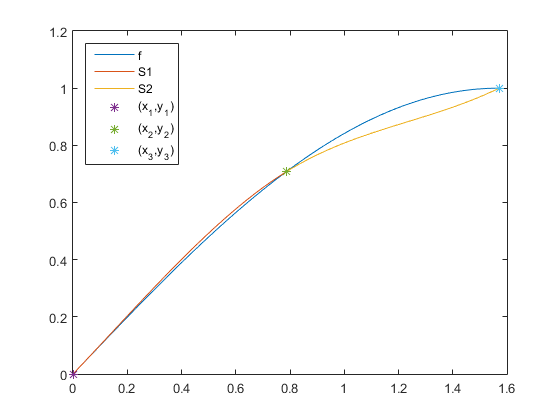
\includegraphics[width=0.5\textwidth]{holmes5_5d.png}
					\caption{Graph of $f(x)$ and clamped cubic splines $S_1(x), S_2(x)$}
				\end{figure} \

			\item Chebyshev interpolation \\

				The function needed to determine the nodes for full-degree interpolation are given by the zeros of the
				Chebyshev polynomial $T_n(x) = cosn\theta$, which occur at $n\theta = \frac{(2k-1)\pi}{2n}$, where $k=1:n$.
				However, this only applies to the interval $[-1,1]$, and therefore must be expanded to our interval $[0,
				\pi/2]$. When generalized, the zeros lie at $\frac{b+a}{2} - \frac{b-a}{2}cos(\frac{(2k-1)\pi}{2n})$, again
				with $k=1:n$. In our case then, $n = 3$, $b = \pi/2$, $a=0$, and the zeros are

				\begin{center}
				\begin{tabular}{ll}
					$k=1$: & $x_1 = \frac{\pi}{4} - \frac{\pi}{4}cos(\frac{\pi}{6}) = 0.1052$ \\
					$k=2$: & $x_2 = \frac{\pi}{4} - \frac{\pi}{4}cos(\frac{\pi}{2}) = \frac{\pi}{4}$ \\
					$k=3$: & $x_3 = \frac{\pi}{4} - \frac{\pi}{4}cos(\frac{5\pi}{6}) = 1.4656$ \\
				\end{tabular}
				\end{center}

				We then use these nodes, to generate a full degree polynomial
				interpolant, in this case using the Lagrange basis.

				$$y = y_1L_1(x_1) + y_2L_2(x_2) + y_3L_3(x_3)$$

				$$L_1(x_1) = \frac{x-\pi/4}{0.1052-\pi/4}*\frac{x-1.4656}{0.1052-1.4656}$$
				$$L_2(x_2) = \frac{x-0.1052}{\pi/4-0.1052}*\frac{x-1.4656}{\pi/4-1.4656}$$
				$$L_3(x_3) = \frac{x-0.1052}{1.4656-0.1052}*\frac{x-\pi/4}{1.4656-\pi/4}$$

				$$y(x) = sin(x_1)L_1(x_1) + sin(x_2)L_2(x_2) + sin(x_3)L_3(x_3)$$

				The function estimate, as well as the error, were calculated through a MATLAB script. The script also plots
				the interpolant and the original function. \\

				$$y(\pi/8) = 0.39790$$
				$$|y(\pi/8)-sin(\pi/8)| = 0.01521$$ \\

				\begin{center}
					\texttt{holmes5\_5e.m} script
				\end{center}
				\lstinputlisting{holmes5_5e.m} \

				\begin{figure}[H]
					\centering
					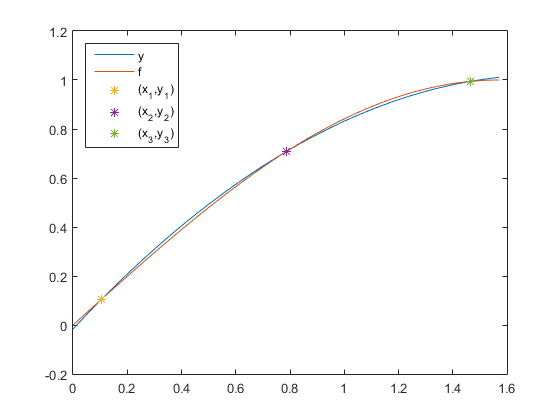
\includegraphics[width=0.5\textwidth]{holmes5_5e.png}
					\caption{Graph of $f(x)$ and the Chebyshev polynomial $y(x)$}
				\end{figure} \

		\end{enumerate}

	\item Function to interpolate: $y(x) = log_{10}x$, where $x\in[0,10]$

		\begin{enumerate}[(a)]

			\item When using a piecewise linear interpolant $p_1(x)$ to approximate a function $f(x)$, the error for a given
				segment from $x_i$ to $x_{i+1}$ is given as
				$$|f(x)-p_1(x)| \leq \frac{1}{2} max|f''(x)|*max|w(x)|$$
				where
				$$w(x) = (x-x_i)(x-x_{i+1})$$
				We can then define the distance between $x_i$ and $x_{i+1}$ as $h$. If we use this definition over the first
				two points in the interpolation $x_1 = 0$, $x_2 = h$, then we can see that $w(x) = (x)(x-h)$, and $w(x)$ will
				reach its maximum magnitude at $x=h/2$, a value of $\frac{h^2}{4}$. This result will hold for not only the
				first interval, but all intervals used for interpolation. Therefore,

				$$|f(x)-p_1(x)| \leq \frac{h^2}{8} max|f''(x)|$$

				We are given the maximum error as $10^{-6}$ and $f(x)$. The only unknown then is a node spacing $h$ that will
				satisfy the inequality.

				$$10^{-6} = \frac{h^2}{8}max|-\frac{1}{x^2log(10)}|$$

				The maximum of $f''(x)$ can be found by the zeros of $f'''(x)$

				$$f'''(x) = \frac{2}{x^3log(10)}$$

				This function has no zeros, so the maximum will occur at one of the ends of the interval $[1,10]$.

				$$|f''(1)| = \frac{1}{log(10)} \approx 0.434294$$
				$$|f''(10)| = \frac{1}{100log(10)} \approx 0.00434294$$

				We now have
				$$10^{-6} = \frac{h^2}{8}*\frac{1}{log(10)}$$
				Solving for $h$, we get $h = \frac{1}{250} \sqrt{\frac{log(10)}{2}}$, which is the largest possible node
				spacing to ensure an error of at most $10^{-6}$. The number of data points then needed to cover the interval
				$[1,10]$ is $9/h = 2250\sqrt{\frac{2}{log(10}}$. Rounding this up, we get
				$$n = 2097$$ \\

			\item A process similar to that of piecewise linear error estimation can be used to estimate the error in a clamped
				cubic spline interpolant. The maximum error of the cubic spline interpolant is given as
				$$|f(x)-S(x)| \leq \frac{3h^4}{384} max|f^{(iv)}(x)|$$
				Here,
				$$|f^{(iv)}(x)| = \frac{6}{x^4log(10)}$$
				which takes its maximum value at $x=1$
				$$|f^{(iv)}(1)| = \frac{6}{log(10)}$$
				We now have everything we need to solve for $h$.

				$$10^{-6} = \frac{3h^4}{384} \frac{6}{log(10)}$$
				$$h \approx 0.033275$$

				The minimum number of nodes for the interval $[1,10]$ is then
				$$\lceil 9/h \rceil = 271$$ \\

			\item The error estimate for a polynomial interpolant given ideal node spacing is
				$$|f(x)-p_n(x)| \leq \frac{1}{2^n(n+1)!} (\frac{b-a}{2})^{n+1}||f^{(n+1)}||_{\infty}$$
				where
				$$||f^{(n+1)}(x)||_{\infty} = max|f^{(n+1)}(x)|,\ x\in[a,b]$$
				and $n$ is the number of data points. This error is not quite as easy to solve, as $n$ is involved in which
				derivative of $f$ is being used, but this can be avoided by realizing the general expression for the
				derivatives of $log_{10}(x)$.

				$$||f^{(n+1)}(x)||_{\infty} = \frac{n!}{x^{n+1}log(10)}$$
				where the maximum will always occur at $x=1$. We now look for values of $n$ such that
				$$10^{-6} = \frac{||f^{(n+1)}(1)||_{\infty}}{2^n(n+1)!}$$
				as this is the smallest possible $n$ that will ensure the error is below the tolerance.

				With some help from the computer, we can now solve for $n$.
				$$\lceil n \rceil = 15$$ \\

		\end{enumerate}

	\item Function to interpolate:
		\[
			g(x)=
			\begin{cases}
				2+3x^2+\alpha x^3 & -1 \leq x \leq 0 \\
				2 + \beta x^2 - x^3 & 0 \leq x \leq 1 \\
			\end{cases}
		\]

		\begin{enumerate}[(a)]

			\item In order for $g(x)$ to be a cubic spline, it must be twice differentiable at $x=0$.
			\[
				g'(x)=
				\begin{cases}
					6x + 3\alpha x^2 & -1 \leq x \leq 0 \\
					2\beta x - 3x^2 & 0 \leq x \leq 1 \\
				\end{cases}
			\]
			\[
				g''(x)=
				\begin{cases}
					6 + 6\alpha x & -1 \leq x \leq 0 \\
					2\beta - 6x & 0 \leq x \leq 1 \\
				\end{cases}
			\]

			\begin{tabular}{lll}
				continuous $g(0)$ & $\to$ & $2 = 2$ \\
				continuous $g'(0)$ & $\to$ & $0 = 0$ \\
				continuous $g''(0)$ & $\to$ & $2\beta = 6$ \\
			\end{tabular} \\

			Based on these results, $\beta = 3$, but $\alpha$ is arbitrary. The two pieces of the function will always be
			not only equal, but will have the same first and second derivatives at $x=0$ as long as $\beta = 3$. We simply choose
			$\alpha = 1$ to keep things simple. The cubic spline through these points is therefore
			\[
				g(x)=
				\begin{cases}
					2+3x^2+x^3 & -1 \leq x \leq 0 \\
					2 + 3x^2 - x^3 & 0 \leq x \leq 1 \\
				\end{cases}
			\] \\

			\item The only data point that was concerning here was the point $x=0$. As there were only two cubic functions making
				up the spline, there is only one point at which they must agree. In this case, that point is $(0,2)$. \\

			\item In order for $g(x)$ to be a natural cubic spline, the second derivatives at each endpoint must be zero. In this
				case, this means
				$$g''(-1) = g''(1) = 0$$
				In other words,
				$$2 + 3(-1)^2 + \alpha (-1)^3 = 0$$
				$$2 + \beta (1)^2 - (-1)^3 = 0$$
				$g(x)$ must still be twice differentiable at $x=0$, so we have added two constraints to the conditions in part
				(a).

				\begin{tabular}{lll}
					$g''(-1) = 0$ & $\to$ & $\alpha = 5$ \\
					$g''(1) = 0$ & $\to$ & $\beta = -3$ \\
					continuous $g(0)$ & $\to$ & $2=2$ \\
					continuous $g'(0)$ & $\to$ & $0=0$ \\
					continuous $g''(0)$ & $\to$ & $2\beta = 6$ \\
				\end{tabular} \\

				We have reached a contradiction, as the definition of a natural spline demands that $\beta = -3$, but the
				conditions for a cubic spline demand that $\beta = 3$. Therefore, there are no values of $\alpha$ and $\beta$
				that make $g(x)$ a natural cubic spline. \\

			\item In order for $g(x)$ to be a clapmed cubic spline, $g'(-1) = f'(-1),\ g'(1) = f'(1)$. However, we are only given
				the function $g(x)$, and not the function that is interpolating. Therefore, we do not know $f'(-1),\ f'(1)$,
				and are left with the same results as part (a). $\beta = 3$, and $\alpha$ is arbitrary. \\

		\end{enumerate}

	\item
		\begin{enumerate}[(a)]

			\item A fairly straightforward MATLAB script was used to calculate the interpolating cubic spline. The script,
				\texttt{holmes5\_16a.m}, stores all given data, and uses the built in \texttt{spline} routine to calculate
				an interpolant that passes through all data points. Next, the \texttt{ppval} routine is used to generate
				a continuous plot of the spline over the entire domain. Included below are both \texttt{holmes5\_16a.m} and
				the graph of the airfoil generated by the script.

				\begin{center}
					\texttt{holmes5\_16a.m}
				\end{center}
				\lstinputlisting{holmes5_16a.m} \

				\begin{figure}[H]
					\centering
					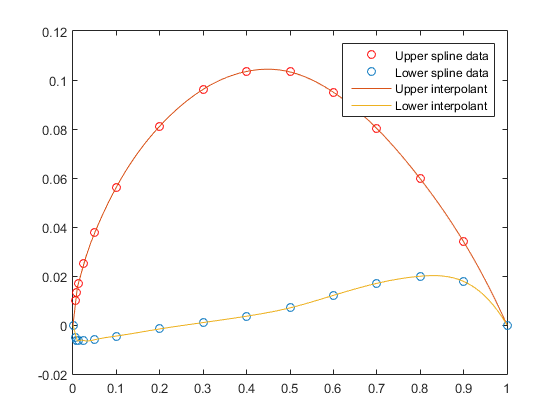
\includegraphics[width=0.6\textwidth]{holmes5_16a.png}
					\caption{Graph of interpolating cubic splines and given discrete data}
				\end{figure} \

			\item Another MATLAB script was used to calculate the full-degree polynomial interpolation of the airfoil. However,
				given the naturally wiggly nature of these interpolants, the resulting graph was completely unrecognizable.
				The initial graph, Figure 10, is the automatically scaled graph of the polynomial from $[0,1]$. Figure 11
				is a zoomed in version, such that the initial data points are still visible.

				\begin{center}
					\texttt{holmes5\_16b.m}
				\end{center}
				\lstinputlisting{holmes5_16b.m} \

				\begin{figure}[H]
					\centering
					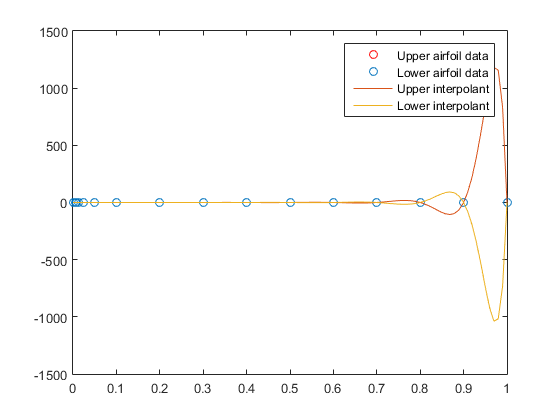
\includegraphics[width=0.6\textwidth]{holmes5_16b_orig.png}
					\caption{Initial graph of interpolating polynomial}
				\end{figure} \

				\begin{figure}[H]
					\centering
					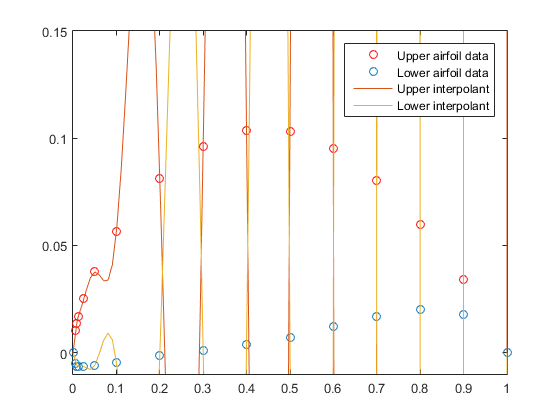
\includegraphics[width=0.6\textwidth]{holmes5_16b_resize.png}
					\caption{Resized graph of interpolating polynomial}
				\end{figure} \

		\end{enumerate}


\end{enumerate}

\end{document}
